% Options for packages loaded elsewhere
\PassOptionsToPackage{unicode}{hyperref}
\PassOptionsToPackage{hyphens}{url}
%
\documentclass[
]{article}
\usepackage{amsmath,amssymb}
\usepackage{lmodern}
\usepackage{iftex}
\ifPDFTeX
  \usepackage[T1]{fontenc}
  \usepackage[utf8]{inputenc}
  \usepackage{textcomp} % provide euro and other symbols
\else % if luatex or xetex
  \usepackage{unicode-math}
  \defaultfontfeatures{Scale=MatchLowercase}
  \defaultfontfeatures[\rmfamily]{Ligatures=TeX,Scale=1}
\fi
% Use upquote if available, for straight quotes in verbatim environments
\IfFileExists{upquote.sty}{\usepackage{upquote}}{}
\IfFileExists{microtype.sty}{% use microtype if available
  \usepackage[]{microtype}
  \UseMicrotypeSet[protrusion]{basicmath} % disable protrusion for tt fonts
}{}
\makeatletter
\@ifundefined{KOMAClassName}{% if non-KOMA class
  \IfFileExists{parskip.sty}{%
    \usepackage{parskip}
  }{% else
    \setlength{\parindent}{0pt}
    \setlength{\parskip}{6pt plus 2pt minus 1pt}}
}{% if KOMA class
  \KOMAoptions{parskip=half}}
\makeatother
\usepackage{xcolor}
\IfFileExists{xurl.sty}{\usepackage{xurl}}{} % add URL line breaks if available
\IfFileExists{bookmark.sty}{\usepackage{bookmark}}{\usepackage{hyperref}}
\hypersetup{
  hidelinks,
  pdfcreator={LaTeX via pandoc}}
\urlstyle{same} % disable monospaced font for URLs
\usepackage{graphicx}
\makeatletter
\def\maxwidth{\ifdim\Gin@nat@width>\linewidth\linewidth\else\Gin@nat@width\fi}
\def\maxheight{\ifdim\Gin@nat@height>\textheight\textheight\else\Gin@nat@height\fi}
\makeatother
% Scale images if necessary, so that they will not overflow the page
% margins by default, and it is still possible to overwrite the defaults
% using explicit options in \includegraphics[width, height, ...]{}
\setkeys{Gin}{width=\maxwidth,height=\maxheight,keepaspectratio}
% Set default figure placement to htbp
\makeatletter
\def\fps@figure{htbp}
\makeatother
\setlength{\emergencystretch}{3em} % prevent overfull lines
\providecommand{\tightlist}{%
  \setlength{\itemsep}{0pt}\setlength{\parskip}{0pt}}
\setcounter{secnumdepth}{-\maxdimen} % remove section numbering
\ifLuaTeX
  \usepackage{selnolig}  % disable illegal ligatures
\fi

\author{}
\date{}

\begin{document}

\begin{titlepage}
  \begin{center}
      \vspace*{1cm}
      \Huge
      \textbf{Math 132A Project 1} \\
      \LARGE
       Auto Assembly
           
      \vspace{1.5cm}
      \large
      \textbf{Teo Zeng}\\
      and\\
      \textbf{Angelica Zheng}
      \vfill
           
           
      \vspace{0.8cm}
  
      \Large
      Department of Mathematics\\
      University of California, Santa Barbara\\
      Febuary 18th, 2023\\
           
  \end{center}
\end{titlepage}

\hypertarget{description-of-the-problem}{%
\section{Description of the
Problem}\label{description-of-the-problem}}

Our company produces different types of automobiles, including trucks,
small cars, and midsized luxury cars. One of the company's plants,
located near Detroit, MI, puts together two kinds of midsized luxury
cars. The first model, known as the Family Adventurer, is a four-door
sedan that comes with standard features, vinyl seats, plastic interior,
and great gas mileage. It is promoted as a wise purchase for
middle-class families who are on a tight budget, and every sale of the
Family Adventurer earns the company a modest profit of 3,700 dollars.
The second model, the Classic Transporter, is a two-door luxury sedan
that has custom features, navigational capabilities, leather seats, and
a wooden interior. It is advertised as a symbol of wealth for
upper-middle-class families, and each sale of the Classic Transporter
generates a profit of 5,300 dollars for the company.

At present we are in the process of determining the manufacturing plan
for the upcoming month. We must make a decision on the number of Family
Adventurers and Classic Transporters to be produced in the plant to
maximize the company's profits. We are aware that the plant has a
labor-hour capacity of 48,500 hours for the month. Additionally, we know
that it takes 6 hours of labor to assemble one Family Adventurer, and
10.5 hours of labor to build one Classic Transporter.

The assembly plant does not manufacture the parts required to put
together the two car models. Instead, these parts are delivered from
other supplier plants located in Michigan. The car parts, such as tires,
windows, doors, steering wheels, and seats, are transported to the
assembly plant. For the upcoming month, William is aware that only
20,000 doors will be obtainable from the door supplier. The doors are
used in both the Family Adventurer and the Classic Transporter, and the
supplier plant was recently impacted by a labor strike, causing the
factory to shut down for a few days. As a result, the supplier plant
will not be able to fulfill its monthly production quota. The 20,000
doors include 10,000 left-hand doors and 10,000 right-hand doors.

Our company has recently projected the monthly demand for various car
models, and the forecast indicates that the demand for the Classic
Transporter will be restricted to 3,500 cars. In contrast, there are no
limits on the demand for the Family Adventurer, as long as the
production capacity of the assembly plant is not exceeded.

\hypertarget{model}{%
\section{Model}\label{model}}

We will use linear programming to model our problem, and we will first
check that our problem satisfies the four assumptions of linear
programming. Let,

\(x_1\) be the number of Family Adventurers to be produced.

\(x_2\) be the number of Classic Transporters to be produced.

\(z\) be the profit to be maximized

Now our decision variable is \(x_1\) and \(x_2\) with objective function
\$ z = 3700x\_1 + 5300x\_2\$

According to the lecture notes, we have

\begin{enumerate}
\def\labelenumi{\arabic{enumi}.}
\tightlist
\item
  \textbf{Proportionality}: which means that each decision variable in
  every equation must appear with a constant coefficient.
\end{enumerate}

\begin{quote}
In our case, proportionality is satisfied because the contribution of
our decision variables to the objective function is proportional to
their values. For example, one Family Adventurer generates a profit of
\(3700\) dollars and two Family Adventurers generate profit of \(7400\)
dollars.
\end{quote}

\begin{enumerate}
\def\labelenumi{\arabic{enumi}.}
\setcounter{enumi}{1}
\tightlist
\item
  \textbf{Additivity}: the combined effect of the decision variables in
  any constraint or in the objective function is the algebraic sum of
  their individual weighted effects.
\end{enumerate}

\begin{quote}
In our case, additivity is satisfied because the contribution to the
objective function for any of our variable is independent of the other
decision variables. For example, the profit of each Family Adventurer
will always be \(3700\) dollars regardless the profit of each Classic
Transporter. And vice versa.
\end{quote}

\begin{enumerate}
\def\labelenumi{\arabic{enumi}.}
\setcounter{enumi}{2}
\tightlist
\item
  \textbf{Divisibility or continuity}: the decision variables can take
  on fractional (non-integer) values.
\end{enumerate}

\begin{quote}
In our case, divisibility is satisfied because when the number of cars
produced are fractional, we can round up or down to obtain an integer
value to satisfy the integer requirement.
\end{quote}

\begin{enumerate}
\def\labelenumi{\arabic{enumi}.}
\setcounter{enumi}{3}
\tightlist
\item
  \textbf{Certainty}: all model parameters (that is, the coefficients of
  the objective function, the coefficients of the constraints) are known
  deterministically (with certainty).
\end{enumerate}

\begin{quote}
In our case, certainty is satisfied because we were given all
constraints, coefficients, objective function of the linear programming
problem, which are all deterministic.
\end{quote}

Having checked that our problem satisfies all four assumption of linear
programming

We formulate our problem as the following \[
\begin{cases}
        \text{Maximize  } \rightarrow z = 3700x_1 + 5300x_2\\
        \text{Subject to:}\\
        6x_1 +10.5x_2 \leq 48500\\
        4x_1 + 2x_2 \leq 20000\\
        x_2 \leq 3500\\
        x_1 \geq 0, x_2 \geq 0
 \end{cases}
\] As we can see in the formulation, we want to maximize the profit
\(z\), which is subject to individual profits of each car model. The
first constraint was due to labor hours. The second constraint was due
to car doors and the third constraint was brought by the company
forecast.

\hypertarget{solution-of-the-model}{%
\section{Solution of the Model}\label{solution-of-the-model}}

Now we will solve the problem using Excel:

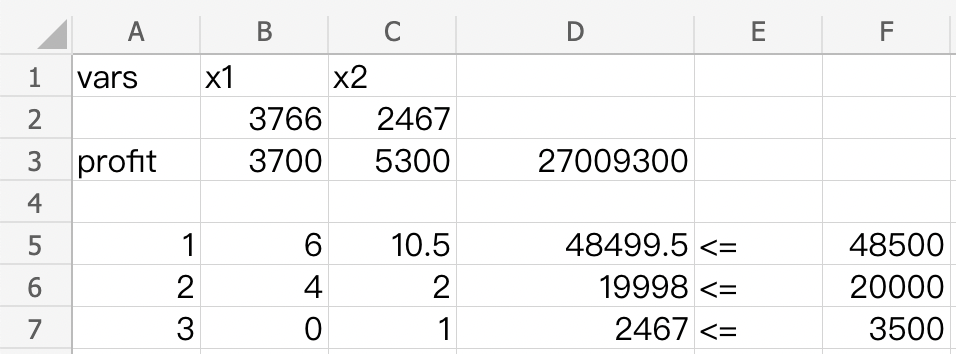
\includegraphics{/Users/teo/Desktop/math132a-project/imgs/excel.png}

We found that the optimal solution is when \[
\begin{cases}
        x_1 = 3766\\ 
        x_2 = 2467
 \end{cases}
\]

\hypertarget{interpretation-of-the-solution}{%
\section{Interpretation of the
Solution}\label{interpretation-of-the-solution}}

The result above means that the objective function is maximized,
satisfying all the constraints, when the company produce \(3766\) Family
Adventurers and \(2467\) Classic Transporters, generating a profit of \[
3700 \times 3766 + 5300 \times 2467 = 27009300 \text{   dollars}
\] To verify that the solution is unique, we plot out the feasible
regions as shown below:

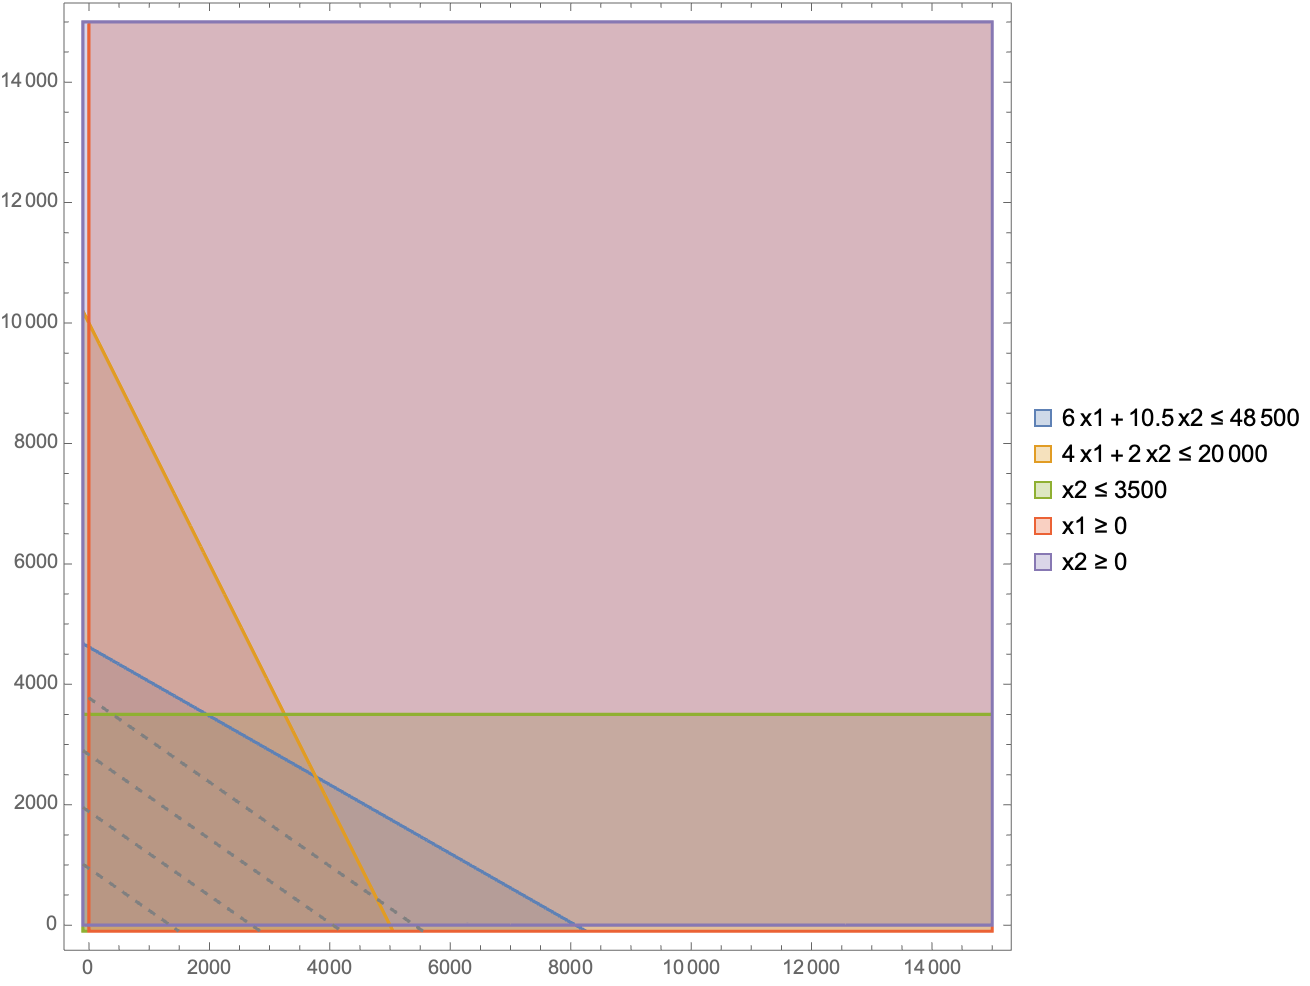
\includegraphics{imgs/plot1.png}

We can see from the above plot, that the conditions form a polygon
boundary. As we increase the objective function \(z\), the dashed line
moved upward. Since the objective function is not parellel to any of the
boundary, there exists an unique optimal to this linear programming
problem. Hence there exists an unique solution.

\hypertarget{recommendation-by-situation}{%
\section{Recommendation by
Situation}\label{recommendation-by-situation}}

The following corresponds to question (3) - (11) in the prompt

\begin{enumerate}
\def\labelenumi{\arabic{enumi}.}
\item
  The marketing department knows that it can pursue a targeted
  \(\$ 500,000\) advertising campaign that will raise the demand for the
  Classic Transporter next month by 20 percent. Should the campaign be
  undertaken?

  Since the target campain cost \(\$ 500000\), this means that we should
  take out \(500000\)\hspace{0pt} in the target function. And since this
  campaign will raise the demand demand for the Classic Transporter next
  month by \(20\) percent, we have the new Linear Programming Problem:
  \[
  \begin{cases}
           \text{Maximize  } \rightarrow z = 3700x_1 + 5300x_2 -500000\\
           \text{Subject to:}\\
           6x_1 +10.5x_2 \leq 48500\\
           4x_1 + 2x_2 \leq 20000\\
           x_2 \leq 4200\\
           x_1 \geq 0, x_2 \geq 0
   \end{cases}
  \] We found that the optimal solution is when \[
  \begin{cases}
           x_1 = 3766\\ 
           x_2 = 2467
   \end{cases}
  \] generating a profit of \[
  3700 \times 3766 + 5300 \times 2467 - 500000 = 26509300 \text{   dollars}
  \] But this is less than the original profit, which is \(27009300\)
  dollars, so William Smith \textbf{should not undertake the campaign.}
\item
  William knows that he can increase next months plant capacity by using
  overtime labor. He can increase the plants labor-hour capacity by 25
  percent. With the new assembly plant capacity, how many Family
  Adventurers and how many Classic Transporters should be assembled?

  Since William Smith can increase the plant capacity by \(25\) percent,
  now he has \(48500 \times 1.25 = 60625\) labor hours. Now we have the
  new linear programming problem: \[
  \begin{cases}
           \text{Maximize  } \rightarrow z = 3700x_1 + 5300x_2\\
           \text{Subject to:}\\
           6x_1 +10.5x_2 \leq 60625\\
           4x_1 + 2x_2 \leq 20000\\
           x_2 \leq 3500\\
           x_1 \geq 0, x_2 \geq 0
   \end{cases}
  \] We found that the optimal solution is when \[
  \begin{cases}
           x_1 = 3250\\ 
           x_2 = 3500
   \end{cases}
  \] generating a profit of \[
  3700 \times 3250 + 5300 \times 3500 = 30575000 \text{   dollars}
  \] Therefore, \textbf{William Smith should now produce \(3250\) Family
  Adventurers and \(3500\) Classic Transporters}.
\item
  William knows that overtime labor does not come without an extra cost.
  What is the maximum amount he should be willing to pay for all
  overtime labor beyond the cost of this labor at regular time rates?

  Without the overtime, the company earns a profit of \(27009300\)
  dollars. With overtime, the company now earns a profit of \(30575000\)
  dollars. \textbf{So the maximum amount of money William Smith would
  like to pay is \(3565700\) dollars.} \[
  30575000 - 27009300 = 3565700 \text{ dollars}
  \]
\item
  William explores the option of using both the targeted advertising
  campaign and the overtime labor-hours. The advertising campaign raises
  the demand for the Classic Transporter by 20 percent, and the overtime
  labor increases the plants labor-hour capacity by 25 percent.
\end{enumerate}

Implementing both advertising and overtime labor will give the new
linear programming problem: \[
  \begin{cases}
        \text{Maximize  } \rightarrow z = 3700x_1 + 5300x_2 - 500000\\
        \text{Subject to:}\\
        6x_1 +10.5x_2 \leq 60625\\
        4x_1 + 2x_2 \leq 20000\\
        x_2 \leq 4200\\
        x_1 \geq 0, x_2 \geq 0
   \end{cases}
  \] We found the solution of this linear programming problem to be \[
  \begin{cases}
        x_1 = 2957\\ 
        x_2 = 4084
   \end{cases}
  \] which generates a profit of \[
  3700 \times 2957 + 5300 \times 4084 - 500000 = 32086100 \text{   dollars}
  \] \textbf{Therefore, William Smith should now produce \(2957\) Family
Adventurers and \(4084\) Classic Transporters}.

\begin{enumerate}
\def\labelenumi{\arabic{enumi}.}
\setcounter{enumi}{4}
\tightlist
\item
  Knowing that the advertising campaign costs \(\$ 500,000\) and the
  maximum usage of overtime labor-hours cost \(\$ 1,600,000\), is the
  solution found in part (6) a wise decision compared to the solution
  found in the beginning?
\end{enumerate}

Since the overtime labor costs \(1600000\) dolars, the new profit for
implementing both advertising and overtime labor yields a profit of \[
  32086100 - 1600000 = 30486100 \text{ dollars}
  \] And we have \(30486100 > 27009300 \text{ dollars}\) we implementing
both \textbf{is a wise decision}.

\begin{enumerate}
\def\labelenumi{\arabic{enumi}.}
\setcounter{enumi}{5}
\item
  The company has determined that dealerships are actually heavily
  discounting the price of the Family Adventurers to move them off the
  lot. Because of a profit-sharing agreement with its dealers, the
  company is therefore not making a profit of \(\$ 3700\) on the Family
  Adventurer but is instead making a profit of \(\$ 2,800\).

  There will be four scenarios. Notice that \textbf{we assume that the
  overtime pay does not cost extra money.}

  \begin{enumerate}
  \def\labelenumii{\arabic{enumii}.}
  \item
    using both advertising and overtime labor

    Now the linear programming problem becomes: \[
    \begin{cases}
          \text{Maximize  } \rightarrow z = 2800x_1 + 5300x_2 -500000\\
          \text{Subject to:}\\
          6x_1 +10.5x_2 \leq 60625\\
          4x_1 + 2x_2 \leq 20000\\
          x_2 \leq 4200\\
          x_1 \geq 0, x_2 \geq 0
     \end{cases}
    \] We found that the solution to this linear programming problem is
    \[
    \begin{cases}
          x_1 = 2754\\ 
          x_2 = 4200
     \end{cases}
    \] generating a profit of \[
    2800 \times 2754 + 5300 \times 4200 - 500000 = 29471200 \text{   dollars}
    \]
  \item
    using overtime labor only

    Now the linear programming problem becomes: \[
    \begin{cases}
          \text{Maximize  } \rightarrow z = 2800x_1 + 5300x_2\\
          \text{Subject to:}\\
          6x_1 +10.5x_2 \leq 60625\\
          4x_1 + 2x_2 \leq 20000\\
          x_2 \leq 3500\\
          x_1 \geq 0, x_2 \geq 0
     \end{cases}
    \] We found that the solution to this linear programming problem is
    \[
    \begin{cases}
          x_1 = 3250\\ 
          x_2 = 3500
     \end{cases}
    \] generating a profit of \[
    2800 \times 3200 + 5300 \times 3500 = 27650000 \text{   dollars}
    \]
  \item
    using advertising only

    Now the linear programming problem becomes: \[
    \begin{cases}
          \text{Maximize  } \rightarrow z = 2800x_1 + 5300x_2 -500000\\
          \text{Subject to:}\\
          6x_1 +10.5x_2 \leq 48500\\
          4x_1 + 2x_2 \leq 20000\\
          x_2 \leq 4200\\
          x_1 \geq 0, x_2 \geq 0
     \end{cases}
    \] We found that the solution to this linear programming problem is
    \[
    \begin{cases}
          x_1 = 735\\ 
          x_2 = 4199
     \end{cases}
    \] generating a profit of \[
    2800 \times 735 + 5300 \times 4199 - 500000 = 23812700 \text{   dollars}
    \]
  \item
    using neither advertising nor overtime labor

    Now the linear programming problem becomes: \[
    \begin{cases}
          \text{Maximize  } \rightarrow z = 2800x_1 + 5300x_2\\
          \text{Subject to:}\\
          6x_1 +10.5x_2 \leq 48500\\
          4x_1 + 2x_2 \leq 20000\\
          x_2 \leq 3500\\
          x_1 \geq 0, x_2 \geq 0
     \end{cases}
    \] We found that the solution to this linear programming problem is
    \[
    \begin{cases}
          x_1 = 1960\\ 
          x_2 = 3499
     \end{cases}
    \] generating a profit of \[
    2800 \times 1960 + 5300 \times 3499 = 24032700 \text{   dollars}
    \]
  \end{enumerate}

  Comparing all four scenarios, option 1 generates a profit of
  \(29471200\) dolloars, which is the most. So William Smith should
  \textbf{consider implenting both advertising and overtime labor.}
\item
  The company has discovered quality problems with the Family Adventurer
  by randomly testing Adventurers at the end of the assembly line.
  Inspectors have discovered that in over 60 percent of the cases, two
  of the four doors on an Adventurer do not seal properly. Because the
  percentage of defective Adventurers determined by the random testing
  is so high, the floor supervisor has decided to perform quality
  control tests on every Adventurer at the end of the line. Because of
  the added tests, the time it takes to assemble one Family Adventurer
  has increased from 6 to \(7.5\) hours.

  With the new time to assemble the Adventurer, assume that William is
  not implementing advertisesment or overtime labor, and the profit of
  adventurer did not drop, we have the linear programming problem as
  follows: \[
  \begin{cases}
           \text{Maximize  } \rightarrow z = 3700x_1 + 5300x_2\\
           \text{Subject to:}\\
           7.5x_1 +10.5x_2 \leq 48500\\
           4x_1 + 2x_2 \leq 20000\\
           x_2 \leq 3500\\
           x_1 \geq 0, x_2 \geq 0
   \end{cases}
  \] We found that the optimal solution is when \[
  \begin{cases}
           x_1 = 1568\\ 
           x_2 = 3499
   \end{cases}
  \] generating a profit of \[
  3700 \times 1568 + 5300 \times 3499 = 24346300 \text{   dollars}
  \] \textbf{Therefore, William Smith should now produce \(1568\) Family
  Adventurers and \(3499\) Classic Transporters}.
\item
  The board of directors of the automobile company wishes to capture a
  larger share of the luxury sedan market and therefore would like to
  meet the full demand for Classic Trasnporters. They ask William to
  determine by how much the profit of his assembly plant would decrease
  as compared to the profit found in part (1). They then ask him to meet
  the full demand for Classic Transporters if the decrease in profit is
  not more than \(\$ 2,000,000\).

  If the full demand of Classic Transporters are met, then the Linear
  Programming Problem becomes: \[
  \begin{cases}
           \text{Maximize  } \rightarrow z = 3700x_1 + 5300x_2\\
           \text{Subject to:}\\
           6x_1 +10.5x_2 \leq 48500\\
           4x_1 + 2x_2 \leq 20000\\
           x_2 = 3500\\
           x_1 \geq 0, x_2 \geq 0
   \end{cases}
  \] We found that the optimal solution is when \[
  \begin{cases}
           x_1 = 1958\\ 
           x_2 = 3500
   \end{cases}
  \] generating a profit of \[
  3700 \times 1958 + 5300 \times 3500 = 25403000 \text{   dollars}
  \] And comparing the profit in (1), \[
  27009300 - 25403000 = 1606300 \text{ dollars} < 2000000 \text{ dollars}
  \] So \textbf{William can meet the full demand.}
\item
  William now makes his final decision by combining all the new
  considerations described in parts (6), (7), and (8). What are his
  final decisions on whether to undertake the advertising campaign?

  Combining all the situations in (6), (7), (8), we formulate the linear
  programming problem as follows: \[
    \begin{cases}
      \text{Maximize  } \rightarrow z = 2800x_1 + 5300x_2 -500000 - 1600000\\
      \text{Subject to:}\\
      6x_1 +10.5x_2 \leq 60625\\
      4x_1 + 2x_2 \leq 20000\\
      x_2 \leq 4200\\
      x_1 \geq 0, x_2 \geq 0
    \end{cases}
  \] We found that the solution to this linear programming problem is \[
    \begin{cases}
      x_1 = 2754\\ 
      x_2 = 4200
    \end{cases}
  \] generating a profit of \[
      2800 \times 2754 + 5300 \times 4200 - 500000 - 1600000= 27871200 \text{   dollars}\\
  \]

  \[
      27871200\text{   dollars} > 27009300\text{   dollars}
  \]

  Since the profit is higher than the original profit based on the
  decisions made in part(6),(7),(8), \textbf{William Smith should now
  produce \(2754\) Family Adventurers and \(4200\) Classic
  Transporters}.
\end{enumerate}

\hypertarget{conclusion}{%
\section{Conclusion}\label{conclusion}}

Given all William Smith's options and possible situations, he should
\textbf{undertake advertisement and use overtime labor} in any
circumstances in order to maximize profit.

\end{document}
